\documentclass[11pt,a4paper]{article}
\usepackage[BoldFont,SlantFont,CJKchecksingle]{xeCJK}
\usepackage{fontspec}
\setmainfont{Courier New}
\usepackage{fontspec}
\setCJKmainfont{WenQuanYi Micro Hei}
\usepackage{xunicode}
\usepackage{xltxtra}
\usepackage{indentfirst}
\XeTeXlinebreaklocale “zh”
\XeTeXlinebreakskip = 0pt plus 1pt minus 0.1pt

\usepackage{ifxetex,ifluatex}
\ifxetex
  \usepackage{fontspec,xltxtra,xunicode}
  \defaultfontfeatures{Mapping=tex-text,Scale=MatchLowercase}
\else
  \ifluatex
    \usepackage{fontspec}
    \defaultfontfeatures{Mapping=tex-text,Scale=MatchLowercase}
  \else
    \usepackage[utf8]{inputenc}
  \fi
\fi
\usepackage{graphicx}
% We will generate all images so they have a width \maxwidth. This means
% that they will get their normal width if they fit onto the page, but
% are scaled down if they would overflow the margins.
\makeatletter
\def\maxwidth{\ifdim\Gin@nat@width>\linewidth\linewidth
\else\Gin@nat@width\fi}
\makeatother
\let\Oldincludegraphics\includegraphics
\renewcommand{\includegraphics}[1]{\Oldincludegraphics[width=\maxwidth]{#1}}
\ifxetex
  \usepackage[setpagesize=false, % page size defined by xetex
              unicode=false, % unicode breaks when used with xetex
              xetex,
              colorlinks=true,
              linkcolor=blue]{hyperref}
\else
  \usepackage[unicode=true,
              colorlinks=true,
              linkcolor=blue]{hyperref}
\fi
\hypersetup{breaklinks=true, pdfborder={0 0 0}}
\setlength{\parindent}{0pt}
\setlength{\parskip}{6pt plus 2pt minus 1pt}
\setlength{\emergencystretch}{3em}  % prevent overfull lines


\usepackage{framed,color}
\definecolor{shadecolor}{gray}{0.95}
\begin{document}

\section{Kmod 运行时调试图}

\subsection{编译安装运行调试图}

\subsubsection{wget下载源码包}

{\begin{shaded}\begin{verbatim}
$ wget https://www.kernel.org/pub/linux/utils/kernel/kmod/kmod-11.tar.gz
--2013-06-18 01:08:47--  https://www.kernel.org/pub/linux/utils/kernel/kmod/kmod-11.tar.gz
Resolving www.kernel.org (www.kernel.org)... 149.20.4.69, 198.145.20.140
Connecting to www.kernel.org (www.kernel.org)|149.20.4.69|:443... connected.
HTTP request sent, awaiting response... 200 OK
Length: 3458574 (3.3M) [application/x-gzip]
Saving to: `kmod-11.tar.gz'

100%[======================================>] 3,458,574    795K/s   in 5.3s    

2013-06-18 01:08:54 (641 KB/s) - `kmod-11.tar.gz' saved [3458574/3458574]
\end{verbatim}\end{shaded}}
\begin{figure}[htbp]
\centering
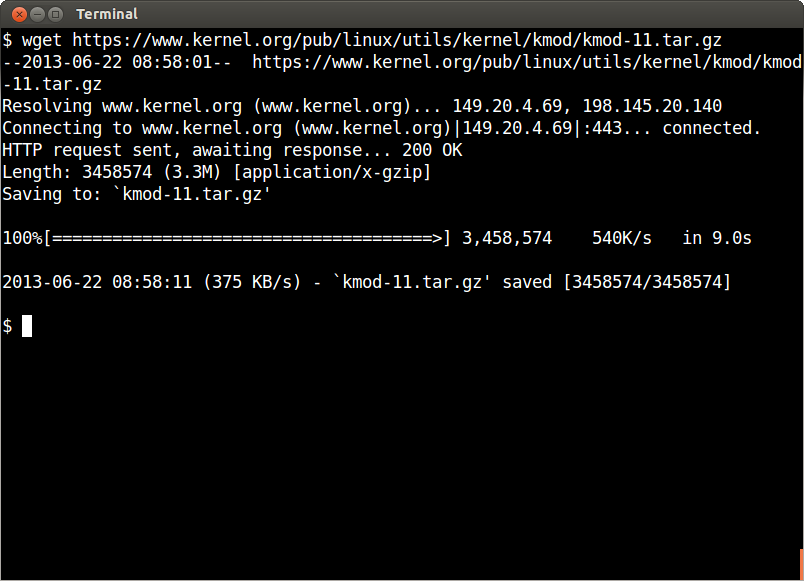
\includegraphics{./pictures/1-1-wget.png}
\caption{wget下载源码包}
\end{figure}

\subsubsection{tar解压源码包}

{\begin{shaded}\begin{verbatim}
$ tar zxf kmod-11.tar.gz 
$ cd kmod-11
$ ls
aclocal.m4   configure     libkmod      Makefile.in  README     tools
build-aux    configure.ac  m4           man          testsuite
config.h.in  COPYING       Makefile.am  NEWS         TODO
$ 
\end{verbatim}\end{shaded}}
\begin{figure}[htbp]
\centering
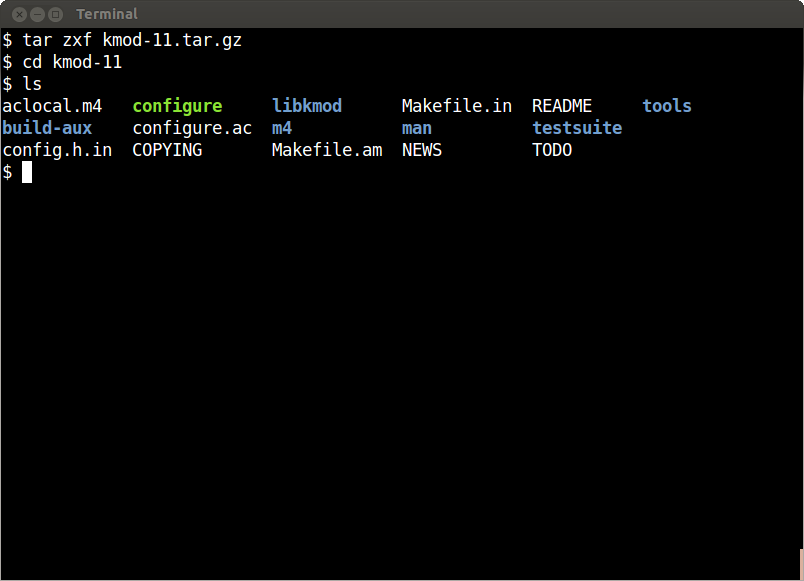
\includegraphics{./pictures/1-2-tar.png}
\caption{tar解压源码包}
\end{figure}

\subsubsection{configure 配置项目源码}

{\begin{shaded}\begin{verbatim}
$ ./configure CFLAGS="-g -O2" --prefix=/usr --sysconfdir=/etc --libdir=/usr/lib
checking for a BSD-compatible install... /usr/bin/install -c
checking whether build environment is sane... yes
checking for a thread-safe mkdir -p... /bin/mkdir -p
checking for gawk... no
checking for mawk... mawk
checking whether make sets $(MAKE)... yes
checking whether make supports nested variables... yes
checking how to create a pax tar archive... gnutar
checking for style of include used by make... GNU
checking for gcc... gcc
checking whether the C compiler works... yes
checking for C compiler default output file name... a.out
checking for suffix of executables... 
checking whether we are cross compiling... no
checking for suffix of object files... o
checking whether we are using the GNU C compiler... yes
checking whether gcc accepts -g... yes
checking for gcc option to accept ISO C89... none needed
checking dependency style of gcc... gcc3
...
kmod 11
======

prefix:         /usr
sysconfdir:     /etc
libdir:         /usr/lib
rootlibdir:     /usr/lib
includedir:     ${prefix}/include
bindir:         ${exec_prefix}/bin

compiler:       gcc -std=gnu99
cflags:          -pipe -DANOTHER_BRICK_IN_THE -Wall -W -Wextra -Wno-inline -Wvla -Wundef -Wformat=2 -Wlogical-op -Wsign-compare -Wformat-security -Wmissing-include-dirs -Wformat-nonliteral -Wold-style-definition -Wpointer-arith -Winit-self -Wdeclaration-after-statement -Wfloat-equal -Wmissing-prototypes -Wstrict-prototypes -Wredundant-decls -Wmissing-declarations -Wmissing-noreturn -Wshadow -Wendif-labels -Wstrict-aliasing=2 -Wwrite-strings -Wno-long-long -Wno-overlength-strings -Wno-unused-parameter -Wno-missing-field-initializers -Wno-unused-result -Wnested-externs -Wchar-subscripts -Wtype-limits -Wuninitialized -fno-common -fdiagnostics-show-option -fvisibility=hidden -ffunction-sections -fdata-sections -g -O2
ldflags:         -Wl,--as-needed -Wl,--gc-sections 

tools:          yes
logging:        yes
compression:        xz=no  zlib=no
debug:          no
doc:            no
man:            yes
\end{verbatim}\end{shaded}}
\begin{figure}[htbp]
\centering
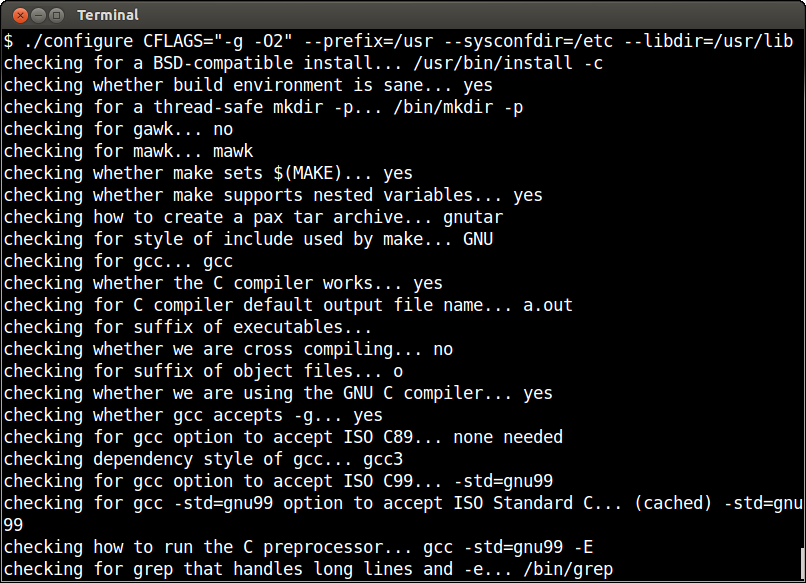
\includegraphics{./pictures/1-3-configure.png}
\caption{configure配置源码包}
\end{figure}

\subsubsection{编译项目源码}

{\begin{shaded}\begin{verbatim}
$ make
make --no-print-directory all-recursive
Making all in .
  CC       libkmod/libkmod.lo
  CC       libkmod/libkmod-list.lo
  CC       libkmod/libkmod-config.lo
  CC       libkmod/libkmod-index.lo
  CC       libkmod/libkmod-module.lo
  CC       libkmod/libkmod-file.lo
  CC       libkmod/libkmod-elf.lo
  CC       libkmod/libkmod-hash.lo
  CC       libkmod/libkmod-array.lo
  CC       libkmod/libkmod-util.lo
  CCLD     libkmod/libkmod-util.la
  CCLD     libkmod/libkmod.la
  CCLD     libkmod/libkmod-private.la
  CC       tools/kmod.o
  CC       tools/lsmod.o
  CC       tools/rmmod.o
  CC       tools/insmod.o
  CC       tools/modinfo.o
  CC       tools/modprobe.o
  CC       tools/depmod.o
  CC       tools/log.o
  CCLD     tools/kmod
  CCLD     tools/kmod-nolib
  GEN      tools/insmod
  GEN      tools/rmmod
  GEN      tools/lsmod
  GEN      tools/modprobe
  GEN      tools/modinfo
  GEN      tools/depmod
  GEN      libkmod/libkmod.pc
Making all in libkmod/docs
make[2]: Nothing to be done for `all'.
Making all in man
make[2]: Nothing to be done for `all'.
\end{verbatim}\end{shaded}}
\begin{figure}[htbp]
\centering
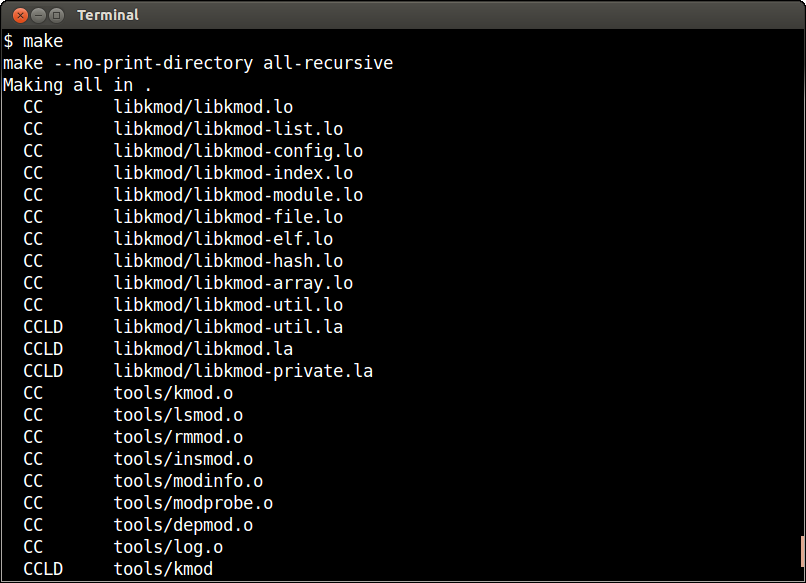
\includegraphics{./pictures/1-4-make.png}
\caption{make编译源码包}
\end{figure}

\subsubsection{测试生成命令}

{\begin{shaded}\begin{verbatim}
$ ./tools/insmod -h
Usage:
    insmod [options] filename [args]
Options:
    -V, --version     show version
    -h, --help        show this help
$ ./tools/rmmod -h
Usage:
    rmmod [options] modulename ...
Options:
    -f, --force       forces a module unload and may crash your
                  machine. This requires Forced Module Removal
                  option in your kernel. DANGEROUS
    -s, --syslog      print to syslog, not stderr
    -v, --verbose     enables more messages
    -V, --version     show version
    -h, --help        show this help
$ ./tools/lsmod -h
Usage: ./tools/lsmod
$ ./tools/modinfo -h
Usage:
    modinfo [options] filename [args]
Options:
    -a, --author                Print only 'author'
    -d, --description           Print only 'description'
    -l, --license               Print only 'license'
    -p, --parameters            Print only 'parm'
    -n, --filename              Print only 'filename'
    -0, --null                  Use \0 instead of \n
    -F, --field=FIELD           Print only provided FIELD
    -k, --set-version=VERSION   Use VERSION instead of `uname -r`
    -b, --basedir=DIR           Use DIR as filesystem root for /lib/modules
    -V, --version               Show version
    -h, --help                  Show this help
$ 
\end{verbatim}\end{shaded}}
\begin{figure}[htbp]
\centering
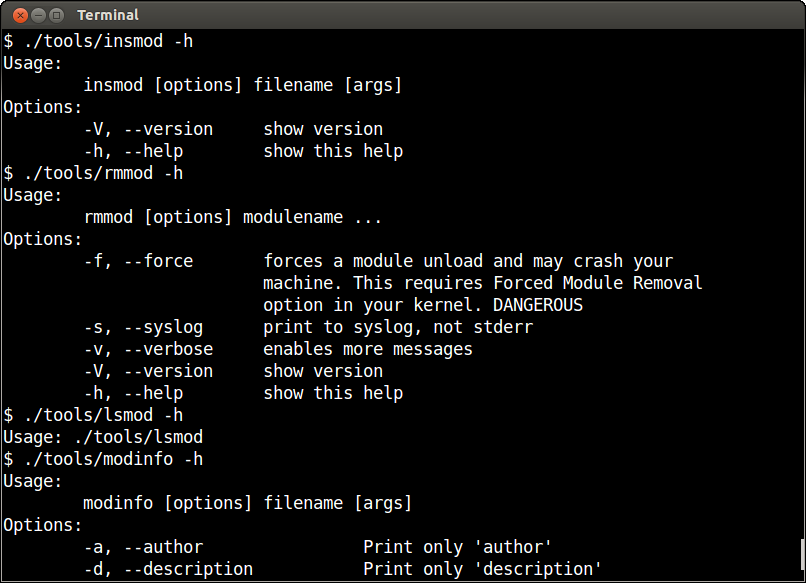
\includegraphics{./pictures/1-5-test.png}
\caption{测试生成命令}
\end{figure}

\subsection{项目Debug版运行调试图}

\subsection{源码修改运行调试图}

\end{document}
